%------------------------------------------------
\section{Desenho e implementação}
%------------------------------------------------

%%%%%%%%%%%%%%%%%%%%%%%%%%%%%%%%%%%%%%%%%%%%%%%%%%%%%%%%%%%
%%%%%%%%%%%%%%%%%%%%%%%%%%%%%%%%%%%%%%%%%%%%%%%%%%%%%%%%%%%
\subsection{Projeto do \textit{hardware}}

\begin{frame}
\frametitle{Desenho e implementação}

Projeto do \textit{Hardware}

\begin{figure}[th]
	\centering
	\captionsetup{width=0.65\textwidth,font=footnotesize,textfont=bf}
	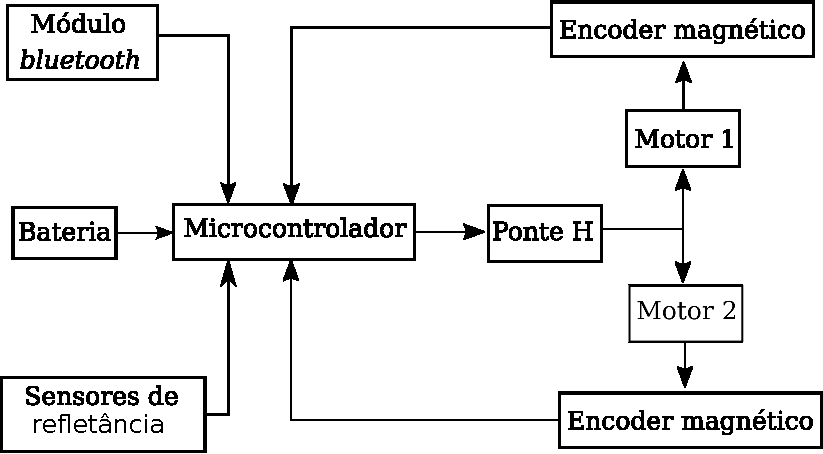
\includegraphics[width=0.65\textwidth,keepaspectratio]{Figuras/DiagramaHW.pdf}
	\caption{Diagrama de funcionamento do \textit{hardware} do veículo.\label{fig:diagEl}}
\end{figure}

\end{frame}

%% ----------------------------------------------------

\begin{frame}
\frametitle{Sensores e condicionamento de sinais}

\begin{figure}[th]
	\centering
	\captionsetup{width=0.65\textwidth,font=footnotesize,textfont=bf}
	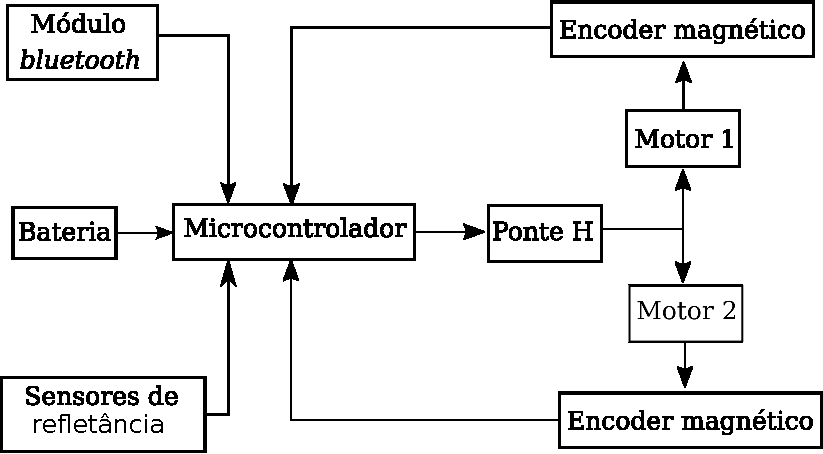
\includegraphics[width=0.65\textwidth,keepaspectratio]{Figuras/DiagramaHW.pdf}
	\caption{Diagrama de funcionamento do \textit{hardware} do veículo.\label{fig:diagEl}}
\end{figure}


\end{frame}

%% To not change the number page of this slide
\begin{frame}[noframenumbering]
\frametitle{Sensores e condicionamento de sinais}



    \transglitter
    \frametitle{Test}
        \begin{itemize}
            \item One
            \item Two
            \item Three
        \end{itemize}
\end{frame}

%% ------------------------------------------------------

\begin{frame}
\frametitle{Sensor de refletância QRE1113}

\begin{figure}[th]
	\centering
	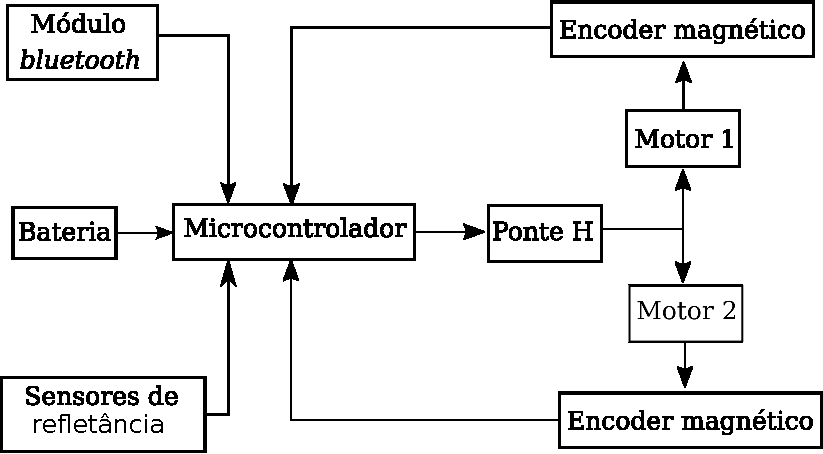
\includegraphics[width=0.65\textwidth,keepaspectratio]{Figuras/DiagramaHW.pdf}
	\caption{Diagrama de funcionamento do \textit{hardware} do veículo.\label{fig:diagEl}}
\end{figure}
\end{frame}

%% ------------------------------------------------------

\begin{frame}
\frametitle{\textit{Driver} de acionamento TB6612FNG}

\begin{figure}[th]
	\centering
	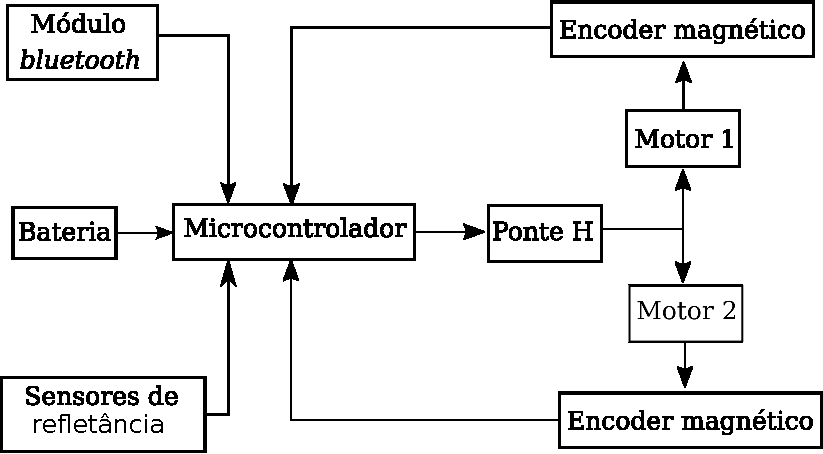
\includegraphics[width=0.65\textwidth,keepaspectratio]{Figuras/DiagramaHW.pdf}
	\caption{Diagrama de funcionamento do \textit{hardware} do veículo.\label{fig:diagEl}}
\end{figure}
\end{frame}

%% ------------------------------------------------------



%%%%%%%%%%%%%%%%%%%%%%%%%%%%%%%%%%%%%%%%%%%%%%%%%%%%%%%%%%%
%%%%%%%%%%%%%%%%%%%%%%%%%%%%%%%%%%%%%%%%%%%%%%%%%%%%%%%%%%%
\subsection{Projeto do controlador de SED}

\begin{frame}
\frametitle{Projeto do controlador de SED}
\begin{columns}
	\column{0.4\linewidth}
		\begin{itemize}
		\item Modelado pelos \textit{softwares} Supremica e Deslab
		\item Autômato de Moore
		\item Variáveis mapeadas:
			\begin{itemize}
			\item B1 (botão);
			\item AcharDir;
			\item PerdeDir;
			\item AchaEsq;
			\item PerdeEsq.
			\end{itemize}
		\end{itemize}
	\column{0.7\linewidth}
		\begin{figure}[th]
		\centering
		\captionsetup{width=\textwidth,font=footnotesize,textfont=bf}
		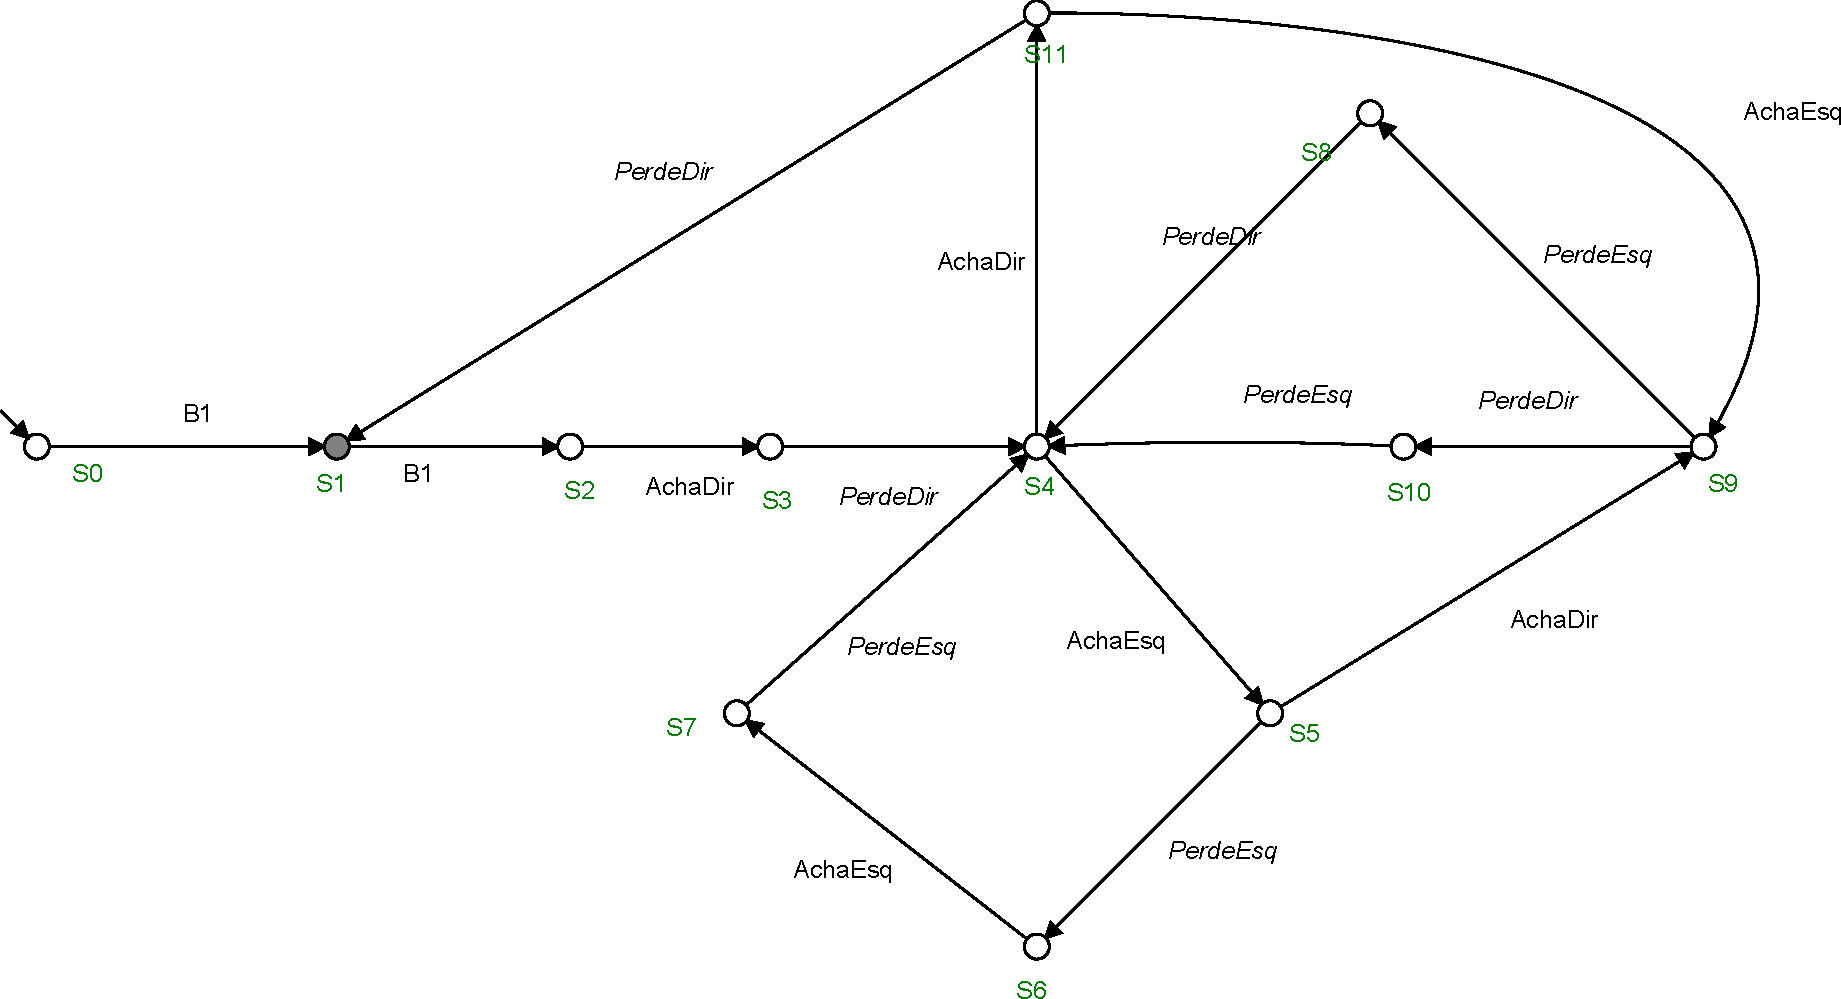
\includegraphics[width=\textwidth,keepaspectratio]{Figuras/SED.pdf}
		\caption{Controlador de SED}				
		\end{figure}
\end{columns}

\end{frame}

%%%%%%%%%%%%%%%%%%%%%%%%%%%%%%%%%%%%%%%%%%%%%%%%%%%%%%%%%%%
%%%%%%%%%%%%%%%%%%%%%%%%%%%%%%%%%%%%%%%%%%%%%%%%%%%%%%%%%%%
\subsection{Projeto do sistema de mapeamento}

\begin{frame}
\frametitle{Projeto do sistema de mapeamento}
\begin{columns}
	\column{0.4\linewidth}
		\begin{itemize}
		\item Modelado pelos \textit{softwares} Supremica e Deslab
		\item Autômato de Moore
		\item Variáveis mapeadas:
			\begin{itemize}
			\item B1 (botão);
			\item AcharDir;
			\item PerdeDir;
			\item AchaEsq;
			\item PerdeEsq.
			\end{itemize}
		\end{itemize}
	\column{0.7\linewidth}
		\begin{figure}[th]
		\centering
		\captionsetup{width=\textwidth,font=footnotesize,textfont=bf}
		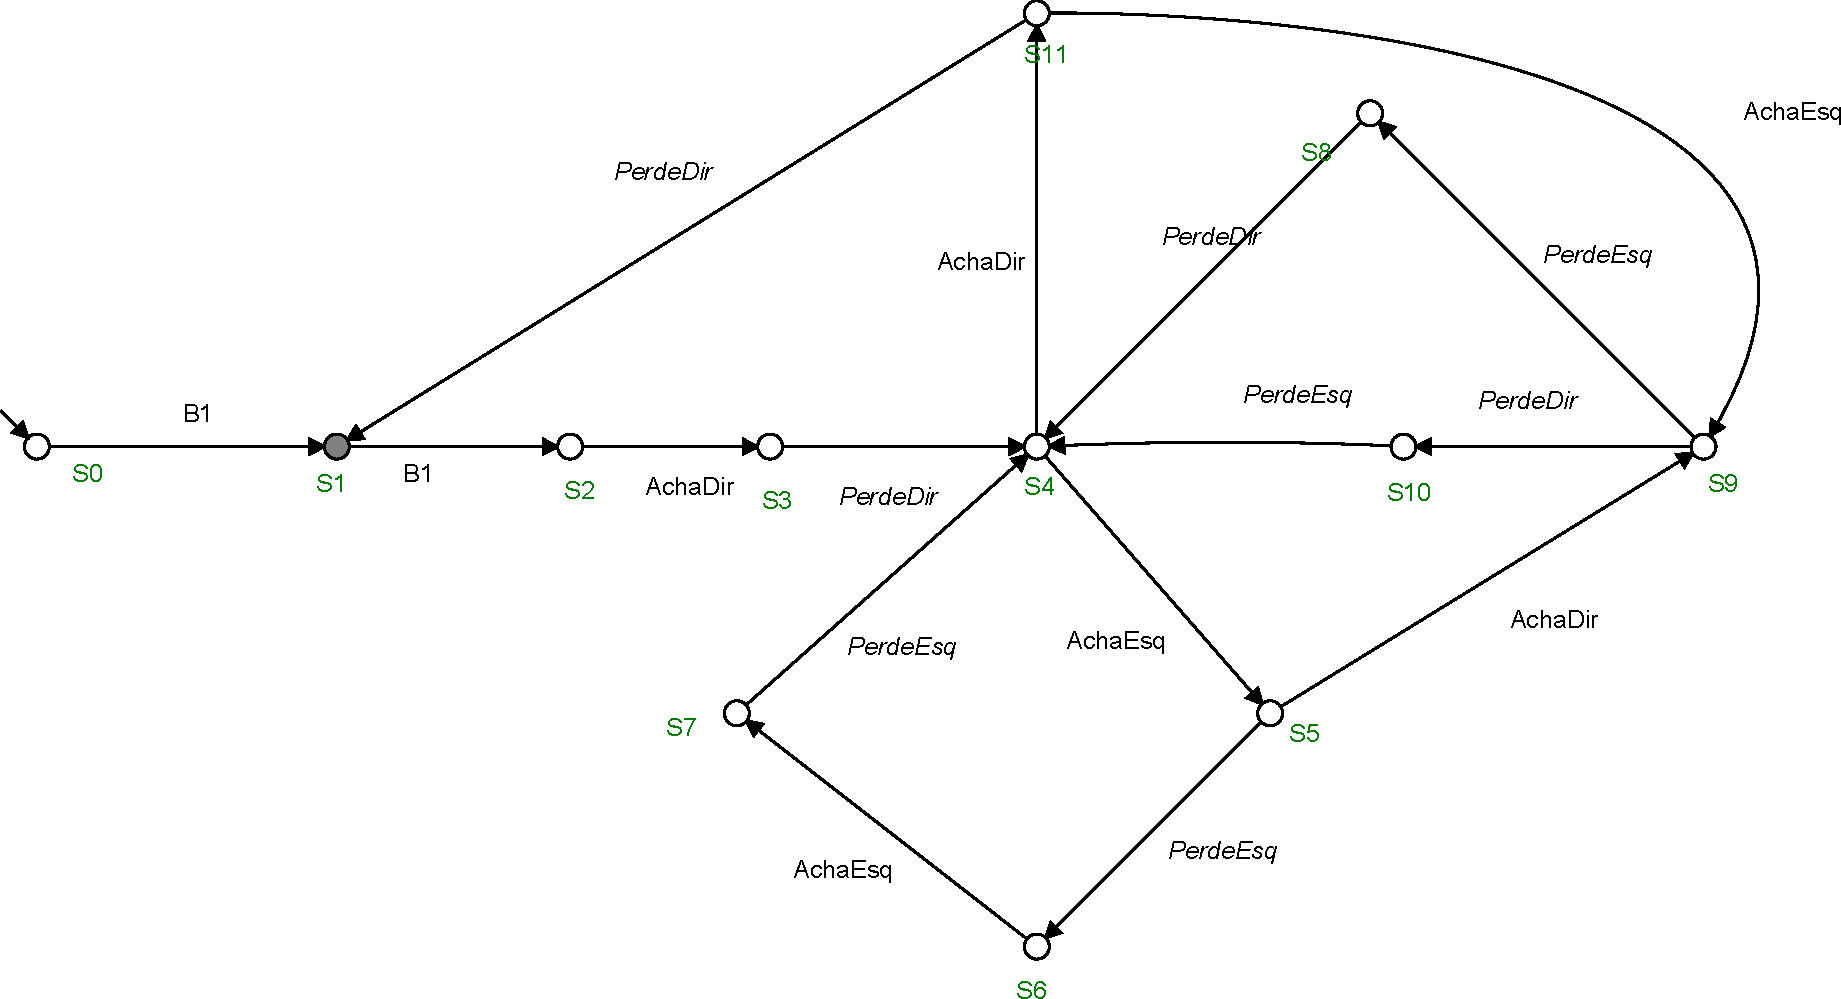
\includegraphics[width=\textwidth,keepaspectratio]{Figuras/SED.pdf}
		\caption{Controlador de SED}				
		\end{figure}
\end{columns}

\end{frame}

%%%%%%%%%%%%%%%%%%%%%%%%%%%%%%%%%%%%%%%%%%%%%%%%%%%%%%%%%%%
%%%%%%%%%%%%%%%%%%%%%%%%%%%%%%%%%%%%%%%%%%%%%%%%%%%%%%%%%%%
\subsection{Função de transferência do veículo}




%%%%%%%%%%%%%%%%%%%%%%%%%%%%%%%%%%%%%%%%%%%%%%%%%%%%%%%%%%%
%%%%%%%%%%%%%%%%%%%%%%%%%%%%%%%%%%%%%%%%%%%%%%%%%%%%%%%%%%%
\subsection{Projeto do controlador de tempo contínuo}















%%% OLD ABOVE %%%%%


\begin{frame}
\frametitle{Table}
\begin{table}
\begin{tabular}{l l l}
\toprule
\textbf{Treatments} & \textbf{Response 1} & \textbf{Response 2}\\
\midrule
Treatment 1 & 0.0003262 & 0.562 \\
Treatment 2 & 0.0015681 & 0.910 \\
Treatment 3 & 0.0009271 & 0.296 \\
\bottomrule
\end{tabular}
\caption{Table caption}
\end{table}
\end{frame}

%------------------------------------------------

\begin{frame}
\frametitle{Theorem}
\begin{theorem}[Mass--energy equivalence]
$E = mc^2$
\end{theorem}
\end{frame}

%------------------------------------------------

\begin{frame}[fragile] % Need to use the fragile option when verbatim is used in the slide
\frametitle{Verbatim}
\begin{example}[Theorem Slide Code]
\begin{verbatim}
\begin{frame}
\frametitle{Theorem}
\begin{theorem}[Mass--energy equivalence]
$E = mc^2$
\end{theorem}
\end{frame}\end{verbatim}
\end{example}
\end{frame}

%------------------------------------------------

\begin{frame}
\frametitle{Figure}
Uncomment the code on this slide to include your own image from the same directory as the template .TeX file.
%\begin{figure}
%\includegraphics[width=0.8\linewidth]{test}
%\end{figure}
\end{frame}

%------------------------------------------------

\begin{frame}[fragile] % Need to use the fragile option when verbatim is used in the slide
\frametitle{Citation}
An example of the \verb|\cite| command to cite within the presentation:\\~

This statement requires citation \cite{p1}.
\end{frame}




%\begin{figure}[H]
%     \centering
%     \captionsetup{width=0.7\textwidth,font=footnotesize,textfont=bf}
%     \begin{subfigure}[b]{\textwidth}
% 	\centering
%         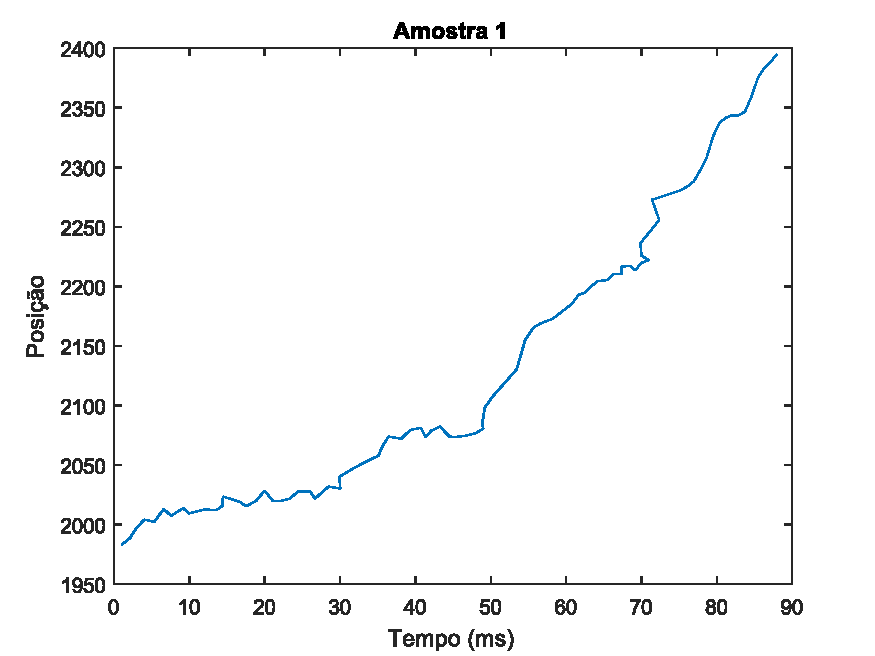
\includegraphics[width=0.6\textwidth,height=\textheight,keepaspectratio]{figuras/Posicao3v2.pdf}
%         \caption{\centering \label{fig:Posicaofinal}}
%     \end{subfigure}
%     
%     \begin{subfigure}[b]{\textwidth}
% 	\centering
%         \includegraphics[width=0.8\textwidth,height=0.3\textheight,keepaspectratio]{figuras/Posicaofinalv2.pdf}
%         \caption{\centering \label{fig:Posicao1}}
%     \end{subfigure}
%
%     \caption{Gráficos da posição em função do tempo (ms), com frequência de 16 KHz e \textit{duty cycle} de 30\%: (a) Amostra 1; (b) Amostra 2 \label{fig:posicoes}}
%     \vspace{-0.3cm}
%     \caption*{Fonte: Autoria própria}
% \end{figure}








%------------------------------------------------

